This section is going through exact details of the process how data was handled and how results were finally obtained.
Actual results are described later on the section~\ref{sec:results-and-discussion}.


\subsection{Initial steps}

To get started with the analysis our Twitter data, we are required to shape data suitable for our use case.
This was briefly described in the section~\ref{sec:dataset-description} on "preprocessing" subsection.
Data was converted into \textbf{.csv} format and loaded into program memory.

Initially, specific Python class was designed to allow ease access for tweet data and feature extraction.
UML diagram can be seen in the figure~\ref{fig:tweetdata_design}.
This class has build-in methods for extracting specific features from the tweet data and it converts values to suitable data types e.g. time into build-in Python time object.
Methods include extracting hashtags, mentions and identification is the tweet retweet, and evaluation of possible sentiment value of it.

\begin{figure}
    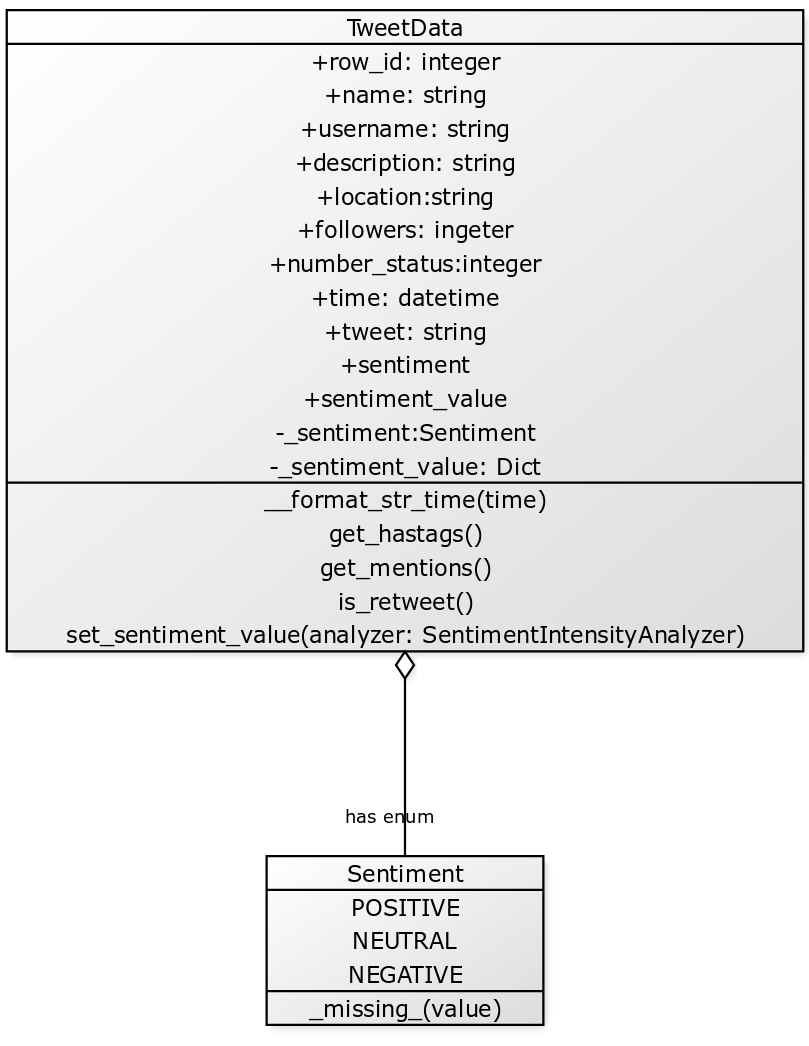
\includegraphics[scale=0.3]{figures/uml_tweetdata}
    \caption{Designed class for storing and handling the Tweet data}
    \label{fig:tweetdata_design}
\end{figure}

Sentiment analysis is used here to make mass analysis for all tweets to categorize every tweet for one of the NEGATIVE, NEUTRAL and POSITIVE semantic orientations.
This is useful stat to generalize what kind message(s) individuals are tweeting.

Individual Twitter users will be sorted and handled separately by using different metrics: by use of the retweets, mentions and use of hashtags.
Also, sentiments among all the tweets will be evaluated.
VADER (Valence  Aware  Dictionary  for  sEntiment  Reasoning) tool\cite{Hutto_Gilbert_2014} has been used for making the sentiment calculation.
It was released in 2014 and has acquired fame from its efficiency and accuracy.
By default, tool is producing four different values for provided input as results.
Three of the values (pos, neu and neg) are pointing the portion of the three orientations, from range to 0 into 1, totalling to sum of 1.
One is describing overall result (compound), which "is computed by summing the valence scores of each word in the lexicon, adjusted according to the rules, and then normalized to be between -1 (most extreme negative) and +1 (most extreme positive)."

Therefore, sentiment orientation is finally defined by compound value as following:

\begin{center}
    \begin{tabular}{ |c|c|c| }
        \hline
        score $\geq$ 0.05 & Positive sentiment \\
        \hline
        score $>$ -0.05 & Neutral sentiment \\
        \hline
        score $\leq$ -0.05 & Negative sentiment \\
        \hline
    \end{tabular}
\end{center}

These threshold values are often used among different researchers and are commonly agreed.
This classification is implemented on the Sentiment enum in the figure~\ref{fig:tweetdata_design}.
It is giving one of the three sentiment description for every tweet based on calculated compound value, automatically.

Ternary plots are used to describe the results, as they often can give clear visual evidence which variable from the three is  the controlling one.
During the assessment of class creation, it was observed that instancing SentimentIntensityAnalyzer from Vader tool is resource consuming, hence
analyzer is instanced only once outside TweetData class and passed into object afterwards to significantly increase performance.


After we have loaded the \textbf{.csv} file, it is parsed in a such a way that from each row in the data, new instance
of TweetData object has been created and list form them is formed.
Further, this list is processed in such a way, that every Twitter user is separated to be part of the new
$<$username$>$:USER\_META dictionary object, which has following attributes; amount\_tweets, amount\_retweets, amount\_mentions, amount\_hashtags and all the tweets this user has tweeted.
This gives us access by username for metadata and user-specific tweets.

Some specific functions have been additionally created that previously created dictionary can be easily sorted, based on it's key-value attributes and finally plotted with suitable graphs.

\subsection{Visualising typical properties}

Now we can plot and sort users based on their amount of tweets, amount of retweets, amount of mentions and by the amount of hashtag usages.
Matplotlib Python package has been used for this.

We are also interested to know, whether power law is applying here, in the context of tweets by single user.
Power law is known to be functional relationship between two quantities, where probability distributions are  "heavy-tailed".
Pareto principle (80-20) is commonly used as rule to see if data fits under power law\cite{enwiki:1023956740}.

Probability distribution of power law can be seen as:

\begin{equation}
    p(x) \propto x^{-\alpha}\label{eq:equation1}
\end{equation}

where $\alpha$ is a constant known usually as scaling parameter and \textit{x} as quantity.
Quantity \textit{x} obeys the power law if it is drawn from this distribution.\cite{doi:10.1137/070710111}

I decided to use specific Python package called as \textbf{powerlaw}\cite{Alstott_2014} for fitting data into distributions and estimating statistical significance.
With powerlaw, data can be fitted into Complementary Cumulative Distribution (CCDF) and compared to theoretical power law, exponential and lognormal distribution candidates.
It has specific function called as \textit{distribution\_compare} which automates a lot of underlying math for calculating two values \textit{R} and \textit{p}.
Mainly Kolmogorov-Smirnov distance algorithm has been used to estimate whether data fits to theoretical estimate.
R is the loglikelihood ratio between the two candidate distributions, which will be positive if the data is more likely in the first distribution.
P value is describing statistical significance of this value.


\subsection{Degree Centrality}

Degree centrality is the sum of in-degree and out-degree.
It is representing the amount of edges entering and leaving the nodes respectively.
The most important nodes have the most direct connections with others under degree centrality.
The value can be computed as,

\begin{equation*}\label{eq:degree-centrality}
C_{D}(v_{i})={\sum}_{j}A_{ij} \tag{1}
\end{equation*}

\subsection{Betweeness Centrality}

Betweeness centrality is another way to measure importance of nodes.
It is describing the amount of the shortest path passing the node.
Important nodes have high betweeness centrality, information is flowing through them, and they are connecting multiple nodes into the network.

\begin{equation*}
    C_{B}(v_{i})={\sum}_{v_{s}\neq v_{i}\neq v_{t}\in V,s < \text{t}}\frac{\sigma_{st}(v_{i})}{\sigma_{st}} \tag{2}
\end{equation*}

